\section{3D Renderer}
The 3D renderer is an uncanny combination of proper 3D techniques and screen space tricks. A summary inspection of its main function (\cw{R\_RenderPlayerView}) reveals it is capable to render three things.\\
\par
\ccode{R_RenderPlayerView.c}{}
\par
\begin{itemize}
	\item Segments (walls and portals which are always vertical).
	\item Flats (ceilings and floors which are always horizontal).
	\item Things (also called "Masked") which are all monsters, weapons, ammo, and sprites in general.
\end{itemize}
 Its most breathtaking aspect of it is its ability to renders walls and flats with zero overdraw. Sprites and Transparent walls do introduce a little bit of overdraw but it is minimal.\\
\par
The full life of a frame can be summarized as follow:
\begin{itemize}
\item Render walls segments, sorted near to far from the player point of view. Both wall ends are projected into screenspace axis X. Based on the distance and floor/ceiling the wall sectors belongs to, calculate a column Y offset and an height. 
\item To render a full wall, generate a set of columns to make ends meet. Interpolate height and Y vertical columns. While rendering:
   \begin{itemize}
     \item record screenspace vertical gaps between walls or between wall and screen boundaries. Infer ceiling (if above mid-screen) or floor (if below miscreen) and stored the area into an array of structure called "visplanes".
     \item Store sprites to be drawn into an array of struct "vissprites".
   \end{itemize}      
\item Render all ceiling and floors from the visplanes.
\item Render transparent elements in far to near order.
\item Render player sprite (the weapon the marine is holding).
\end{itemize}
\par
The most important part (and what \doom engine is most famous for) is the ability to sort walls and things extremely efficiently thanks to its Binary Space Partition tree. Interestingly, there is a bit of a back story about how the BSP came to be a central part of the game engine.\\
\par
\pagebreak
%\trivia{Wolfenstein 3D and Doom have orthogonal architectures. Where the former tried to draw everything vertically to favor the VGA, the latter tried to draw everything horizontally to favor the 486 cachelines.}

% \subsection{Walls}
% There are two ways to render walls in a correct way. Either go with a painter algorithm which draw far to near and involves no book-keeping but generate a lot of overdraw. Or draw near to far, keeping track of what has been drawn which is more compicated but has zero overdraw. In both strategy lies the problem of sorting them according to the player point of view. Given the high cost of rendition, \doom went for the latter approach.\\
% \par

% \subsubsection{Sorting walls}
In its early instance the engine consumed exactly what the designer produced, namely lines and sectors. Starting in the sector containing the player, the engine would look for double sided lines and treat them as portals, traversing the map in a near to far fashion. Each portal lead to adjacent sector where the process was repeated recursively\footnote{That was the same design Ken Silverman's build engine would settle on to power Duke Nukem 3D. However in 1996 Pentium had taken over and were more than able to deal with complex polygons.}.\\
\par
\srawpngdrawing{0.7}{duke_map}
\vspace{1cm}
\fq{The engine was built out of "sectors" -- complex polygonal regions with a common floor / ceiling texture and height, but it didn't have the BSP-chopped "subsectors".  It started in the view sector and recursively flowed into the adjourning sectors, but because they could all be complex polygons it was a lot of record keeping to know what parts you had already visited or were in the stack somewhere.  It worked, and simple areas were fast, but it slowed down precipitously with complexity.}{John Carmack}
\par
Things indeed slowed down significantly with a particular map of John Romero creation.\\
\par
\fq{I was working on E1M2 around April 1993, and I created a set of circular stairs. John C. wrote the renderer with a sector list to know what should be rendered. The problem is that this set of stairs made his sector list building code take a really long amount of time to execute because the same sectors needed to be put into the list over and over due to how the algorithm worked.}{John Romero}\\
\par
\fullimage{SCREEN01.png}%{Notice the HUD using a huge portion of the 3D canvas.} 
\label{HUD_screenshot}
\par
As the news that the technology was not good enough to ship, around the same time an other very serious issue arose.\\
\par
Back in August 1992, id Software had landed a contract with Nintendo to port Wolfenstein 3D to SNES. They subcontracted the project and forgot about it to focus on \doom. In April 1994, the contractor was nowhere in sight. They had nothing to deliver to Nintendo. It was a big deal involving a huge penalty.\\
\par
 Development for \doom stopped completely as the team desperately banged they old game together into a machine not remotely built to do what they wanted. While Tom Halls dusted of his 6502 assembly skills, John Carmack had a different kind of problem at hand, the raycasting technology which Wolfenstein relied on was too much for the Nintendo console. The SNES and its 6503 on steroids simply did not have enough juice for the DDA algorithm\footnote{You can read everything about DDA in Game Engine Black Book: Wolfenstein 3D}.\\% It turned out a white paper co-authored by Bruce Naylor would end up making a huge difference.\\
\par



\fq{John started searching around for 3D research papers. He had several VHS tapes of math conferences, and compendiums of graphics papers from conferences because game books were a rare thing back then, and there was nothing printed that could help us create the engine we were building -- he had to figure out where to get information that was not directly applicable to games and figure out how to adapt it to his problem.\\
\par
Bruce Naylor's May 1993 AT\&T Bell Labs paper was titled "Constructing Good Partitioning Trees" and was published in the proceedings of Graphics Interface '93. John had this book in his collection. Bruce's explanation of BSPs was mostly to cull backfaces from 3D models, but the algorithm seemed like the right direction, so John adapted it for Wolfenstein 3D.}{John Romero}\\
\par
\fq{I do remember clearly that I first used BSP for the SNES version of Wolfenstein, which was a gentle introduction with everything being axial and easier to visualize, which gave me more confidence I would be able to make it work when I went back to working on Doom}{John Carmack}\\
% Concave and convex sectors proved to be too much complexity for the engine to deal with and maintain a descent frame rate. This was a huge issue. They did not have much time to work on it thought, since around the same time this issue was discovered, work on \doom had to stop in order to respond to an emergency.\\
% \par
With a visual surface determination not based on raycasting but rather on BSP, Wolfenstein 3D SNES managed to reach an acceptable framerate\footnote{}. Within three weeks the managed to produce "something".\\
\par
Due to Nintendo strict non-violence policy the game had to be heavily censored to reach a child-friendly quality. Blood was replaced with sweat. guard dogs are replaced with mutant rats and Hitler was renamed "Staatmeister" (which translates to State Master).\\
\par
And with that problem solved, by the end of April, the whole team was back on \doom.
\pagebreak

\cfullimage{bsp_paper.png}{Bruce Naylor's paper: "Constructing Good Partitioning Trees"}
\pagebreak

\subsection{Binary Space Partitioning: Theory}
Binary Space Partitioning trees have many applications. The one we are interested in is how \doom uses them to perform VSD (Visible Surface Determination). Bruce Naylor's thesis paper "ON VISIBLE SURFACE GENERATION BY A PRIORITI TREE STRUCTURES" features a pretty good summary.\\

 \begin{verbatim}
In order to determine the visible surface at each pixel, traditionally
tile distance from the viewing position to each polygon which maps onto 
that pixel is calculated. Most methods attempt to minimize the number 
of polygons to be so considered. Our approach eliminates these distance
calculations entirely. Rather, it transforms the polygonal data base 
(splitting polygons when necessary) into a binary tree which can be 
traversed at image generation time to yield a visible priority z value
for each polygon.
\end{verbatim}

\par
\fq{When I did the early work on BSPs\footnote{That was while working on Quake, John and Bruce met only after \doom shipped.}, Bruce Naylor came down and visited here and gave me copies of a bunch of his papers. It's interesting to talk to people about the old days. Of course, you've got the Internet now. You can find anything nowadays. But back then, it was really something to get reprints of old academic papers. There were some clearinghouses I used to use: you'd pay twenty-five dollars or whatever, and they'd mail you xeroxes of old research papers. It was just a very, very different world. I learned most of my programming when I had a grand total of like three reference books. You had to figure everything else yourself. So I was finding I was reinventing a lot of classic things, like Huffman encoding or LZW encoding. So I'd be all proud of myself for having figured something out, and then I'd find it was just classic method and they did it better than I did.}{John Carmack, Interview for Scarydarkfast}\\
\par
To understand how BSPs work, let's take the example of a map which could easily have been created with DoomED.\\
\par
 For simplicity the map we will be working with is made of eight vertices linked together to form a room made of four walls (\cw{A}, \cw{B}, \cw{C}, and \cw{D}). Inside the room a pillar which is also made of four walls (\cw{E}, \cw{F}, \cw{G}, and \cw{G}). The map is made of only one complex sector (it has a hole in it). Despite is simplicity it is obvious how it is a difficult problem to solve to a renderer since depending on the point of view the order in which the wall must be drawn will vary. A naive solution would require a complex sorting algorithm. Notice that all lines have a direction and all lines have only one side (on their right side).\\

\par
\rawdrawing{doom_map}
\par
To build the BSP from the map, the core idea is to repeatedly select a line to spit the map in two. Split lines become \cw{SEGMENTS} and split sectors become {SUB-SECTORS}.\\ 
\par
In our example, a list of poor choices of splitters would be \cw{A}, then \cw{B}, \cw{C}, and \cw{D} since they would not divide data well.\\ 
\par
Let's say our heuristic selected line \cw{H} which conveniently cut  the room in half. Some lines are entirely on the left of H and some are entirely on its right. Lines on both sides must be slit into segments.  After the split, the two leaves in the BSP contains two sub-sectors. One is convex (\cw{\{A, B1, H D1\}}) and will not be touched anymore. The other one is concave (\cw{\{E, F, G, B2, C, D2\}}) and will need further splitting. The process is repeated until all subsectors are convex.\\
\par
\drawing{doom_map_split1}{}
\par
The process is repeated until every node is reduced to a convex sub-space. Notice how the binary tree grows, with splitting plan as nodes and segments in the leave. 
\par
\rawdrawing{doom_map_split2}
\par
At this point in the splitting we are still not done. The area between \cw{B2}, \cw{C2}, \cw{F}, and \cw{F} is concave. We need one last split.\\ 
\par
\drawing{doom_map_split3}{}
\par
With all sub-sectors in the leave convex, the BSP construction ends. The number of vertices and segments to deal has increased by 50\% but we now have a data structure capable of sorting all segments, from any point of view, at the cost of only three comparison.\\
\rawdrawing{doom_map_split4}
\par
This is only one of the many possible trees which could have been generated with the map. Choosing splitters in an alphabetical order would have produced an inefficient BSP.\\




\rawdrawing{doom_map_bad}{}
\par

\subsubsection{Usage}

\begin{wrapfigure}[10]{r}{0.5\textwidth}
\centering
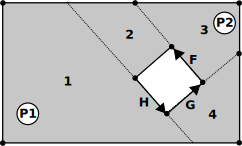
\includegraphics[width=.5\textwidth]{drawings/doom_map_walk.pdf}
\end{wrapfigure}
To use the BSP, we only need to traverse it depth first and choose a branch based on a position on the map. Let's take two example using the BSP in figure XXX. For convenience of notation, sub-sectors have been labeled \cw{1} to \cw{4} and only the splitting lines are marked.\\
\par
From point of view \cw{P1}, traversing the BSP takes three tests. \cw{P1} is on the right of \cw{H}, on the left of \cw{G}, and on the left of \cw{F}. Which give the order near to far: \cw{1,2,3,4}. Notice that once the subsector is determined, it doesn't matter what order segments within a subsector are drawn since all subsectors are convex.\\
\par
From point of view \cw{P2}, traversing the BSP also takes three tests. \cw{P2} is on the left of \cw{H}, on the left of \cw{G}, and on the left of \cw{F}. Which give the order near to far: \cw{3,2,4,1}.\\
\par
The beauty of binary trees is that traversing them is a constant cost. No matter where we try to place the player on the map, it will always take three tests to sort all subsectors and their segments.
\pagebreak




\subsection{Binary Space Partitioning: Practice}
For \doom~, maps were preprocessed on a NeXTStation Turbo via the in-house tool node builder named \cw{doombsp}.\\
\par
For the tool to build the best BSP possible a splitter selection heuristic had to be established. A good splitter divides the map as evenly as possible (and therefore limit the depth of the tree) and is either horizontal or vertical (to be easier to debug).\\
\par
 \cw{doombsp} recursively inspect all lines in a subspace and give a splitting score to each of them. At the end of the evaluation, the highest scoring line is selected. Map is split in two and the process is repeated until only convex subsectors remain. This is a CPU intensive task which took XXXs for a E1M1 featured in Figure \ref{E1M1_lines}. And a total of XXX for all thirty maps of \cw{DOOM.WAD}.\\
\par
\drawing{E1M1_lines}{E1M1, a.k.a Episode 1 Map 1.}
\par
Figure \ref{E1M1_segs} shows the seven first splitters selected on E1M1. First level in red, second level in blue and the third level in green.\\
\par
Switching from sectors flooring to Binary Space Partition not only cost preprocessing time and frustration to map designers. There was a second side effect which was much more of an issue since it affected the players. Because the BSP sliced the map and created new vertices, wall positions was set in stone, there was no way to move walls.

\drawing{E1M1_segs}{Seven first splitters in the E1M1 BSP}
\drawing{E1M1_fab}{All subsectors at the end of E1M1 tree construction, each is a convex leaf.}

\par


\subsection{Drawing Walls}
With the expert knowledge of BSP in mind, we can take a look at the first step of a scene rendition. Namely, to render walls. No surprise here, \cw{R\_RenderBSPNode} traverses the tree near to far and send sub-sectors found to be rendered.\\
\par
\ccode{R_RenderBSPNode.c}
\par


To perform the side test, any geometry book will describe how to represent the plan with a parametric equation $$ P = P0 + t * (P1 - P0) $$
and use the power of the dot product to inject the coordinate of the test point, essentially projecting the point on a line perpendicular to the plan. The sign of the result tell if the point is in front or in the back of the plan.\\
\par
This technique is far from optimal since it requires either floating point or fixed point arithmetic. There is a better way which involves not the magic of the dot product but the awesomeness of the cross product.\\
\par
\ccode{R_PointOnSide.c}
\pagebreak


\begin{wrapfigure}[8]{r}{0.25\textwidth}
\centering
\includegraphics[width=.25\textwidth]{drawings/line_cross_product.png}
\end{wrapfigure}
Notice in the previous code listing how nodes are not stored as coordinate of two vertices \cw{Point 1}, \cw{Point 2} but rather as \cw{Point 1}, \cw{Delta to Point 2}. This storage technique made the cross-product faster to generate since one of the vector (from the node) was already calculated.\\
\par


\subsubsection{Wall Projection}
We are not down in \cw{R\_Subsector} function where all segments in a subsectors are rendered in order. This part of the pipeline relies heavily on BAM (Binary Angular Measurement) where degrees in interval \cw{[0, 360]} are mapped in the full range of a 32-bit integer.\\
\par
\ccode{bam.c}
\par
The angle of both end of the segment with respect to the player position are calculated. Segment with a negative angle (angleP2 - angleP2 < 0) are culled since they are not facing the camera. Segment passing the angle test are projected onto the screen via a double translation table. First the BAM is reduced from 32-bit to 13-bit. Then the angle is injected into a lookup table \cw{viewangletox} to give a screepspace \cw{X} coordinate.\\
 \par

\pngdrawing{projectionExplained}{}
\par
\cw{viewangletox} is generated to give the player 90 degree angle of vision and project to the border of the screen anything else. 
\par
\pngdrawing{angletoxTable}{}
\par
With the sector floor and height a column dimension and vertical offset are calculated. With the distance to the player, scaling is applied. At this point the engine has the dimension of both ends of a segment calculated. But it is not time to draw yet. A little bit of clipping must occur. 






\subsubsection{Wall Clipping}
At this point, we need to differentiate two types of segments. Segments with only one side (connected with only one sector) which are opaque and I will call walls. Segments with two sides (connecting two sectors) which are often transparent in the middle and which I will call portals.\\
\par
Clipping is a two steps process happening in screen space. The first, crude, step is horizontally based. Only walls affects the horizontal occlusion array but all segments are clipped against it.\\
\par
The second, fine, step is vertically based. Both walls and portals affects the vertical occlusion array and both are clipped against it.\\
\par
\pagebreak

\subsubsection{Horizontal Crude Wall Clipping}
The pass maintains a \cw{solidseg} array which keeps track of the walls horizontal occlusion. Since portal can be seen through, they have no impact on \cw{solidseg}. Since walls can be split due to occlusion, this pass output was is called "fragments".\\
\par
\ccode{hclipper.c}
\par
Let's take a simple example and proceed step by step. In the room below, the player is facing north and four walls need to be rendered.
\par
\rawpngdrawing{clip_map}
\par

Initially the occlusion array has two entry, one representing what is on the left of the screen, from infinity to -1 and one on the right of the screen from 320 to infinity.\\
\par 
\begin{minipage}{0.54\textwidth}
\centering
\ccode{clip0.c}
\end{minipage}
\begin{minipage}{0.46\textwidth}
\centering
\srawpngdrawing{0.95}{clip0}
\end{minipage}
\par






The first wall is rendered. There is nothing to occlud it and it is in the middle of the screen. A entry is added to represent the occlusion state.\\
\par
\begin{minipage}{0.54\textwidth}
\centering
\ccode{clip1.c}
\end{minipage}
\begin{minipage}{0.46\textwidth}
\centering
\srawpngdrawing{0.95}{clip1}
\end{minipage}
\par



The second wall is rendered. Its left side is clamped via angle adjustment and the right side if not occluded. Since it touch the left edge of the screen no entry in the occlusion array is added.
\par
\begin{minipage}{0.54\textwidth}
\centering
\ccode{clip2.c}
\end{minipage}
\begin{minipage}{0.45\textwidth}
\centering
\srawpngdrawing{0.95}{clip2}
\end{minipage}
\par





The third wall is rendered. It happens to lie just next to the second wall. It is fully converted to a wall fragment and nothing is discarded. The occlusion array is updated
\begin{minipage}{0.54\textwidth}
\centering
\ccode{clip3.c}
\end{minipage}
\begin{minipage}{0.46\textwidth}
\centering
\srawpngdrawing{0.95}{clip3}
\end{minipage}
\par


Finally the last wall is rendered. While occluded against the array, it is slipt into two fragments. The occlusion array is updated. All segment ended up touching each others. 
\begin{minipage}{0.54\textwidth}
\centering
\ccode{clip4.c}
\end{minipage}
\begin{minipage}{0.46\textwidth}
\centering
\srawpngdrawing{0.95}{clip4}
\end{minipage}
\par

\subsubsection{Vertical Fine Wall Clipping}
The second pass clips fragments vertically. A data structure based on two arrays as wide as the 3D canvas is maintained. While walls will mark a column as completely occluded, portals will only update the occlusion columns with what their upper and lower part cover.\\
\par
\ccode{vclippers.c}
\par
Let's take an other example with a simple room with two portal in the middle. Walls \cw{A}, \cw{C}, and \cw{D} mark the occlusion column fully while portal \cw{B} makes clipping limit progress toward the screen center.
\pagebreak

At the end of this step, fragments are converted into columns which are passed to the rasterizer \cw{colfunc()}
\pagebreak


\subsubsection{Wall drawing}
Interpolation
\trivia{To play nicely with cachelines (at least for read operations), texture data are stored as column major (rotated 90degrees left).}













\subsection{Flats}
At this point in the rendering pipeline, the framebuffer \#1 looks like mashed potatoes. A scene that would end up looking this way:\\
\par
\fullimage{mashed_potatoes1.png}
\par
As been partially drawn like this:\\
\fullimage{mashed_potatoes2.png}
\par

 All walls are correct but there are huge gaps in between which need to be filled. This is where the visplanes are used. How floors and ceilings are drawn is the most difficult part to understand. The puzzled command in the source code "Now what is a visplane, anyway?" tells a lot about the mystery surrounding them.\\
\par
\ccode{visplanes.c}
\par
In a nutshell, a visplane stores the screen space area of a ceiling or a floor which needs to be drawn. A modified version of the engine, drawing visplane in plain color help to visualize them.\\
\par
\fullimage{doom_visplanes.png}{}\\
\fullimage{doom_visplanes_colored.png}{} 22 visplanes
%\fullimage{doom_visplanes_colored_merged.png}{} 6 visplanes
\par
The previous screenshot was slightly misleading in order to ease comprehension. There are fourteen visplanes in that screenshot which is a lot for a simple room with a window. It is a problem in terms of memory consumption since a \cw{visplane\_t} struct is no less than 664 bytes. 9 KiB off storage for such a simple screen but imagine a scene with a staircase and two windows and the number of visplane could easily climb to 100s which would consum way too much for a game already struggling to fit into 4 MiB.\\
\par
To solve this problem, the engine merges visplanes as they are encountered. If two visplanes share the same texture, height, light intensity and if they don't overlad vertically, they are merged. In the previous example this brings the fourteen visplanes figure down to five.\\
\par
\fullimage{doom_visplanes_colored.png}{}
\fullimage{108visplanes.png}{}

\par
\begin{verbatim}
sizeof(visplane) = 664
(664) * 128 = 84992
framebuffers
\end{verbatim}
\fullimage{many_visplanes.png}




















\subsection{Visplanes and DrawPlanes overflow}
Even with visplane merging, the number of visplanes could still get out of hand. Storage was not dynamic, it was capped at 128 units. If the engine encountered condition where 129 visplanes were required it would quit with the following mysterious message:\\
\begin{verbatim}
"R\_FindPlane: no more visplanes"\\
\end{verbatim}
\par
R\_DrawPlanes: visplane overflow (\%i)\\
R\_DrawPlanes: drawsegs overflow (\%i)\\
R\_DrawPlanes: opening  overflow (\%i)"\\
\par

\trivia{The limitation on 128 visplanes was not only necessary to fit within the memory budget, it was also a runtime necessity. When attempting to merge visplanes, the engine search complexity algorithm based on a linear search, making it a $O(n^})$ operation which would become a bottleneck as the number of visplanes increased. In 1997, Lee Killough lifted this limitation, replacing linear search with a $O(1)$ chained hash table\footnote{Source: The Truth about Visplane Overflows}.
\par
\ccode{visplane_linear_search.c}




\subsection{Diminishing Lighting}
\label{diminishedlightning}
\begin{wrapfigure}[11]{r}{0.33\textwidth}
\centering
\scaledimage{0.33}{palette.png}
\end{wrapfigure}
So far our trip down the rendering pipeline assumed that values from the texture and sprite texels were used as is, indexing colors from the palette. That made things easier to understand but now is time to introduce diminished lightning.\\
\par
With the VGA, the mode Y allowed only 256 colors but as it turned out there was a smart way to fake more colors than available. Artists were allowed to use the full 256 primary colors and still get 32 shade of each without requiering $256 * 32 = 8192$ colors.\\
\par
 The trick to fake more colors than available is to reorganize the initial palette of 256 colors and for each values, try to use one of the other 255 available to fake 32 shades toward black. For some colors like skin, red, green, grey, brown or red it worked very well. For others not so much but given the speed of the game the human eye was forgiving.\\
 \par
 The trick implementation starts with a lump called \cw{COLORMAP} which looks like figure XX. The original palette indexes are unrolled in the first column. Fifteen additional columns are appended to the left of each colors. Notice that even though it may look like it has more, figure XXX only features 256 colors.\\
\par
In the source code, each column is refered to as a "lightmap". Before drawing starts, a lightmap column pointer is selected which acts as an indirection layer between the color in the asset and the shaded color to be rendered.\\
\par
\ccode{lightmap.c}
\par
The lightmap selection algorithm is different based on one of the three types of things renderered.\\
\par
\begin{itemize}
\item Wall. dc\_colormap = walllights[index]; where index 
\item Flat: start at sector light level [0,16] -> planezlight. index based on distance [0,128] ds\_colormap = planezlight[index];\\ lighttable\_t*    zlight[LIGHTLEVELS][MAXLIGHTZ]; How is zlight initialized?
\item Masked.
\end{itemize}
\par
\cscaledimage{1}{COLORMAP.png}{COLORMAP and its 32 lightmaps.}
\par




\cw{COLORMAP} contains a 17th lightmap made of 256 shades of grey. It is used when the player picks up the invulnerability bonus.\
\par 
\fullimage{idbeholdv.png}
\par
This trick turned out to be a nightmware to replicate when developers ported \doom to hardware accelerated machines which where RGB based and not palette based. With OpenGL an exotic \cw{glBlendFunc(GL\_ONE\_MINUS\_DST\_COLOR, GL\_ZERO)} was usually attempted to give a result that was pretty close.\\
\par
\fullimage{invOpenGL.png}
\par
Play with:
\begin{verbatim}
player->fixedcolormap
\end{verbatim}


TODO: With and witout screenshot\\
\par
TODO: With and witout screenshot2\\
\par
trivia: colormap hacks. Doom EGA and Doom CGA.\\





\section{Door}
Door code to make them open horizontally.
\section{Texture Mapping}
Persepctive correct was too expensive. But since only one axis had to be corrected, there was a way to get away with fast affine texture mapping.\\
https://www.doomworld.com/forum/topic/86977-doom-affine-texture-mapping-edition/\\
\par



\section{Masked}
Things, masked walls and player sprite.\\

\null\newpage % Make toc appear on right side
\par

\scaledimage{0.25}{cacodemon1.png}\scaledimage{0.25}{cacodemon2.png}\scaledimage{0.25}{cacodemon3.png}\scaledimage{0.25}{cacodemon4.png}\\

\scaledimage{0.25}{cacodemon9.png}\scaledimage{0.25}{cacodemon10.png}\scaledimage{0.25}{cacodemon11.png}\scaledimage{0.25}{cacodemon12.png}\\

\scaledimage{0.25}{cacodemon17.png}\scaledimage{0.25}{cacodemon18.png}\scaledimage{0.25}{cacodemon19.png}\scaledimage{0.25}{cacodemon20.png}\\

\scaledimage{0.25}{cacodemon25.png}\scaledimage{0.25}{cacodemon26.png}\scaledimage{0.25}{cacodemon27.png}\scaledimage{0.25}{cacodemon28.png}\\

\pagebreak

\scaledimage{0.25}{cacodemon5.png}\scaledimage{0.25}{cacodemon6.png}\scaledimage{0.25}{cacodemon7.png}\scaledimage{0.25}{cacodemon8.png}\\

\scaledimage{0.25}{cacodemon13.png}\scaledimage{0.25}{cacodemon14.png}\scaledimage{0.25}{cacodemon15.png}\scaledimage{0.25}{cacodemon16.png}\\

\scaledimage{0.25}{cacodemon21.png}\scaledimage{0.25}{cacodemon22.png}\scaledimage{0.25}{cacodemon23.png}\scaledimage{0.25}{cacodemon24.png}\\

\scaledimage{0.25}{cacodemon29.png}\scaledimage{0.25}{cacodemon30.png}\scaledimage{0.25}{cacodemon31.png}\scaledimage{0.25}{cacodemon32.png}\\

\par

\subsection{Things}
\begin{verbatim}
vissprite_t	vissprites[MAXVISSPRITES];

typedef struct vissprite_s {
    
    struct vissprite_s*	prev; // Doubly linked list.
    struct vissprite_s*	next;
    
    int			x1;
    int			x2;
    
    fixed_t		gx; // for line side calculation
    fixed_t		gy;		

    fixed_t		gz; // global bottom / top for silhouette clipping
    fixed_t		gzt;

    fixed_t		startfrac;     // horizontal position of x1
    
    fixed_t		scale;
        
    fixed_t		xiscale;	 // negative if flipped

    fixed_t		texturemid;
    int			patch;

    // for color translation and shadow draw,
    //  maxbright frames as well
    lighttable_t*	colormap;
   
    int			mobjflags;
    
} vissprite_t;

// While wall rendering, generate structure able to build a sprite clipping.
drawseg_t	drawsegs[MAXDRAWSEGS];
drawseg_t*	ds_p;

short clipbot[SCREENWIDTH];
short cliptop[SCREENWIDTH];

\end{verbatim}

Clipping is done via \cw{drawseg\_t	drawsegs[MAXDRAWSEGS];} array which is as big as the max \# of walls rendered.\\
\par
Drawing is done as columns: \cw{R\_DrawMaskedColumn}. Sprites are stored to please cachelines in reading.







\subsection{Weapon}

\subsection{Pot pourri}
The early 1993 press release written by Tom Halls (see Annexe page \pageref{label_press_release}) made some bold statements. Besides promising the best game of all time, it was remarquably accurate with regards to features the 3D renderer would end up shipping with:\\
\par
\par
Some of the annouced features had already been achieved by John Carmack. The game engine he had written during his research and licensed to Shadowcaster\footnote{See more details about Shadowcaster on page \pageref{label_shadowcaster}.} featured a fully texture mapped environement including flats (walls and ceilings). Light dminishing was also relatively easily implemented. However non-orthogonal walls was a big promise.\\
\par
\trivia{Three Screen Mode}
